\section{Result I: Added Structure Gives No Detectable Gain over a Matched Flat Model}
\label{sec:result1}
In all four collections, no structured model beats the matched flat model. The scope differs by
collection: on xla:default both arms are learning-rate tuned; on nlp:default both run at a matched 1e-4
(exploratory); on xla:random and nlp:random all arms share 1e-3; and the hierarchical model was tested
only on the xla collections. The one result that looked like a clear win, on xla:default, did not
survive the pre-registered baseline check.

\subsection{xla:random: no gain from hierarchy or contention edges}
\label{sec:xla-random}
The hierarchical model does not beat the parameter-matched flat model: $\tau = 0.2645 \pm 0.0230$
against $0.2880 \pm 0.0365$, $\Delta\tau = -0.0235 \pm 0.0214$ ($p = .07$), with a point estimate that
leans negative. The contention-edge model scores $0.2640 \pm 0.0360$, $\Delta\tau = -0.0241 \pm
0.0665$ ($p = .46$); its large seed spread puts the MDE near 0.11. Top-$K$ slowdown is also null at
every $K$ (all $p \geq .45$), so neither model improves the configurations an autotuner would actually
try. On the convolution graphs' Top-1, the metric of Section~\ref{sec:capstone}, neither model differs
from flat either (hierarchical $+0.022$, $p = .77$; contention-edge $+0.003$, $p = .97$; MDE about
0.27). We checked the edge construction against a dense reference implementation, which agreed to
within 1e-7. Checkpoints were chosen at evaluation batch 32 but scored at batch 8; 12 of the 15 chosen
checkpoints are from the final epoch, and the conclusions hold at both batches.

\subsection{nlp:random: contention edges are marginally worse}
\label{sec:nlp-random}
On nlp:random's 20 validation graphs, the contention-edge model is marginally worse than flat:
$\tau = 0.6408 \pm 0.0334$ against $0.7129 \pm 0.0577$, $\Delta\tau = -0.0722 \pm 0.0583$
($p = .0504$). Top-$K$ agrees at $K = 5$ and 10 and is not significant at $K = 1$ or 100. Both arms
share lr 1e-3 and this model is learning-rate sensitive, so an under-tuned contention-edge model is a
possible explanation.

\subsection{xla:default: an apparent large win at the shared learning rate}
\label{sec:xla-default}
At the shared lr of 1e-3, both connectivity models appear to beat the flat model by a wide margin
(Figure~\ref{fig:staircase}). The flat baseline scores $\tau = 0.0327 \pm 0.0135$, the hierarchical
model $0.1484 \pm 0.0276$ and the contention-edge model $0.1977 \pm 0.0133$, so contention-edge $-$
flat is $\Delta\tau = +0.1650 \pm 0.0133$ ($p < .001$). The contention-edge model wins on all five
seeds, the margin is about 12 times the seed spread, the arms are parameter-matched, and the result
survives Benjamini--Hochberg correction. It passes audit Axes 1--3 and most papers would report it as
a win. One graph carries much of it (inception\_v3, $\Delta\tau$ $+0.550$; the other six average
$+0.101$), and Appendix~A decomposes the gain into hierarchy and edge components. The warning sign is
the flat model itself: $\tau = 0.033$ is barely better than random ranking ($\tau = 0$).

\begin{figure}[t]
\centering
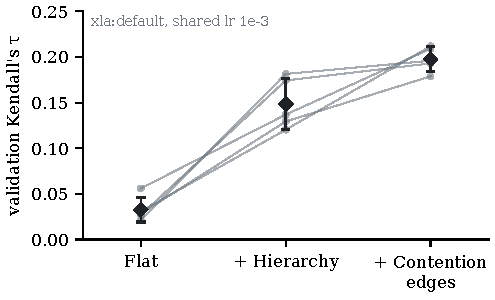
\includegraphics[width=\columnwidth]{figures/fig_r1_xla_default_staircase.pdf}
\caption{At a shared learning rate of 1e-3, adding hierarchy and then contention edges appears to raise
validation Kendall's $\tau$ on xla:default from 0.033 to 0.198. Grey lines join the five paired seeds;
black markers show mean $\pm$ std (evaluation batch 8). Section~\ref{sec:tuning} shows that the rise
comes from an untuned flat baseline.}
\label{fig:staircase}
\end{figure}

\subsection{Tuning the baseline dissolves the win}
\label{sec:tuning}
We trained each model at five learning rates (3e-5, 1e-4, 3e-4, 1e-3 and 3e-3) and kept each model's
best by validation $\tau$ (Figure~\ref{fig:lr}). The flat model is best at 1e-4 and collapses at 1e-3,
the shared rate. Against the tuned flat baseline, the contention-edge model at 1e-3 is no longer a win
(though not significantly worse), and the hierarchical model is worse. With both arms tuned, the
contention-edge model is also best at 1e-4 and no difference is detected: $\Delta\tau = +0.002$
($p = .88$, MDE 0.037). Tuning raised the flat model by $+0.193$ $\tau$ but the contention-edge model by
only $+0.029$, so the original $+0.165$ was mostly the flat model being held back. The best rates were
picked on the same validation set that is scored, within a 50-epoch budget in which most runs peaked at
epoch 46 or later; both limitations apply equally to both arms.

We call this the baseline-strength pattern: a gain measured against an untuned baseline that shrinks
below detection once the baseline is tuned. It recurs twice in Section~\ref{sec:capstone}.

\begin{figure}[t]
\centering
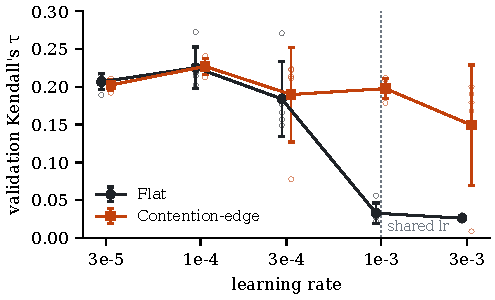
\includegraphics[width=\columnwidth]{figures/fig_r4_lr_curves.pdf}
\caption{Validation $\tau$ on xla:default at five learning rates for the flat and contention-edge
models (open circles: seeds; filled: mean $\pm$ std; 50-epoch budget). The flat model's collapse at the
shared rate of 1e-3 (dashed line) produces the apparent gain in Figure~\ref{fig:staircase}; at each
model's best rate the two are indistinguishable.}
\label{fig:lr}
\end{figure}

\subsection{nlp:default: a training failure, then an amended run}
\label{sec:nlp-default}
At the shared lr of 1e-3, the contention-edge model did not train on nlp:default: from the first epoch
it gave every layout the same score (seeds 42 and 100), so $\tau$ is undefined on all 20 validation
graphs. We recorded this as a training failure before reading the relevant results (Amendment~1,
Appendix~B); it says nothing about the information the graph carries. An exploratory rerun of both arms
at 1e-4, a rate chosen after seeing the failure, finds no difference: $\tau = 0.4087$ against flat's
$0.4138$, $\Delta\tau = -0.0051$ ($p = .53$, MDE 0.027). Compared with flat at the untuned 1e-3, the
contention-edge model would have looked like a winner ($+0.089$, $p = .02$), but flat itself gains
$+0.095$ from the lower rate. Across collections, the apparent advantages come from the learning rate,
not the connectivity. We next ask where the remaining error lies.
